\section{Redes neuronales prealimentadas
profundas}\label{redes-neuronales-prealimentadas-profundas}

\label{sec:feedforward}

Las redes prealimentadas profundas, también conocidas como perceptrones
multicapa o en inglés como \emph{deep feedforward neural networks}, son
el modelo canónico de aprendizaje profundo \autocite{goodfellow2016}. El
objetivo de una red prealimentada es aproximar una función \(f^{*}\),
definiendo una aplicación \(f(x;\theta)\) y aprendiendo el valor de los
parámetros \(\theta\) que resultan en la mejor aproximación.

En concreto, las redes prealimentadas se caracterizan por que no se
forman ciclos en las conexiones entre unidades. Así, la información se
evalúa siempre hacia adelante a través de las conexiones intermedias
usadas para definir \(f\), hasta la salida de la red. No hay
retroalimentaciones en las que salidas de algunas unidades de la red
vuelvan a ser entradas del modelo.

Estas redes se suelen representar como una composición en cadena de
varias funciones, que se puede asociar a un grafo acíclico. Por ejemplo,
podríamos tener una red composición de funciones vectoriales
\(f_1, f_2, f_3\) de la siguiente forma: \(f(x)=f_3(f_2(f_1(x)))\). En
este caso, decimos que \(f_1\) es la primera capa, \(f_2\) la segunda
capa y \(f_3\) la capa de salida. Las capas que no corresponden a la
salida de \(f\) se suelen denominar \emph{capas ocultas}. La longitud de
esta cadena nos da la profundidad del modelo.

A diferencia de otros algoritmos de aprendizaje automático, las redes
neuronales mantienen esta estructura de capas de forma que la capa
\(i+1\)-ésima únicamente opera con los datos de salida de la
\(i\)-ésima; en particular, sólo la primera capa utiliza directamente
los datos de entrada. Además, por la inspiración biológica de las redes,
cada componente de cada capa (\emph{unidad}) se puede interpretar como
una neurona, actuando como una función de \(\RR^{n_{i-1}}\) en \(\RR\),
donde \(n_{i-1}\) es el número de componentes de la capa anterior. El
comportamiento es similar a una neurona en el sentido de que recoge
información de varias unidades cercanas y calcula su propio valor de
activación, así como la estructuración en capas se ha tomado de la
neurociencia. En la figura \ref{fig:dfnn} se muestra una representación
común de una red neuronal como unidades conectadas formando un grafo.
Las flechas indican el sentido en el que viajan los datos, es decir, las
salidas de funciones que se toman como entradas de otras funciones.

\begin{figure}[hbtp]
  \centering
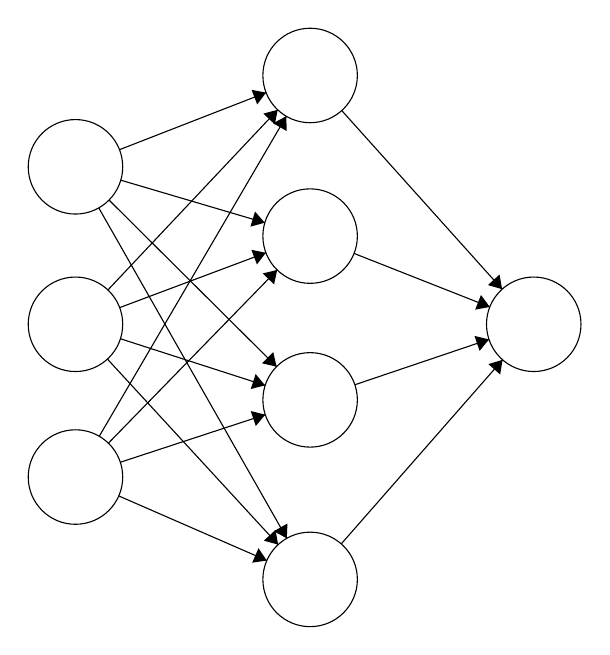
\begin{tikzpicture}[scale=0.2]
\tikzstyle{every node}+=[inner sep=0pt]
\draw [black] (21.5,-13.4) circle (3);
\draw [black] (21.5,-23.4) circle (3);
\draw [black] (21.5,-33.1) circle (3);
\draw [black] (36.4,-7.6) circle (3);
\draw [black] (36.4,-17.8) circle (3);
\draw [black] (36.4,-28.2) circle (3);
\draw [black] (36.4,-39.6) circle (3);
\draw [black] (50.6,-23.4) circle (3);
\draw [black] (24.35,-32.16) -- (33.55,-29.14);
\fill [black] (33.55,-29.14) -- (32.63,-28.91) -- (32.95,-29.86);
\draw [black] (24.25,-34.3) -- (33.65,-38.4);
\fill [black] (33.65,-38.4) -- (33.12,-37.62) -- (32.72,-38.54);
\draw [black] (23.59,-30.95) -- (34.31,-19.95);
\fill [black] (34.31,-19.95) -- (33.39,-20.17) -- (34.11,-20.87);
\draw [black] (23.01,-30.51) -- (34.89,-10.19);
\fill [black] (34.89,-10.19) -- (34.05,-10.63) -- (34.91,-11.13);
\draw [black] (23.56,-21.22) -- (34.34,-9.78);
\fill [black] (34.34,-9.78) -- (33.43,-10.02) -- (34.16,-10.71);
\draw [black] (24.31,-22.34) -- (33.59,-18.86);
\fill [black] (33.59,-18.86) -- (32.67,-18.67) -- (33.02,-19.6);
\draw [black] (24.36,-24.32) -- (33.54,-27.28);
\fill [black] (33.54,-27.28) -- (32.94,-26.56) -- (32.63,-27.51);
\draw [black] (23.53,-25.61) -- (34.37,-37.39);
\fill [black] (34.37,-37.39) -- (34.2,-36.46) -- (33.46,-37.14);
\draw [black] (24.3,-12.31) -- (33.6,-8.69);
\fill [black] (33.6,-8.69) -- (32.68,-8.51) -- (33.04,-9.44);
\draw [black] (24.38,-14.25) -- (33.52,-16.95);
\fill [black] (33.52,-16.95) -- (32.9,-16.24) -- (32.61,-17.2);
\draw [black] (23.63,-15.51) -- (34.27,-26.09);
\fill [black] (34.27,-26.09) -- (34.06,-25.17) -- (33.35,-25.88);
\draw [black] (22.98,-16.01) -- (34.92,-36.99);
\fill [black] (34.92,-36.99) -- (34.96,-36.05) -- (34.09,-36.54);
\draw [black] (38.41,-9.83) -- (48.59,-21.17);
\fill [black] (48.59,-21.17) -- (48.43,-20.24) -- (47.69,-20.91);
\draw [black] (39.19,-18.9) -- (47.81,-22.3);
\fill [black] (47.81,-22.3) -- (47.25,-21.54) -- (46.88,-22.47);
\draw [black] (39.24,-27.24) -- (47.76,-24.36);
\fill [black] (47.76,-24.36) -- (46.84,-24.14) -- (47.16,-25.09);
\draw [black] (38.38,-37.34) -- (48.62,-25.66);
\fill [black] (48.62,-25.66) -- (47.72,-25.93) -- (48.47,-26.59);
\end{tikzpicture}
\caption{\label{fig:dfnn} Ilustración ejemplificando una red neuronal prealimentada de tres capas}
\end{figure}

Para entender cómo las redes prealimentadas aproximan funciones,
consideremos algunos modelos lineales como la regresión lineal o la
logística. Estos modelos tienen claras ventajas, son sencillos, se
pueden ajustar de forma eficiente y fiable. Sin embargo, están muy
limitados, dado que sólo tiene sentido aplicarlos a funciones lineales,
por lo que no pueden sintetizar interacciones entre dos variables de
entrada.

Cuando el objetivo es aproximar funciones no lineales, una vía es
aplicar un modelo lineal no a la variable independiente sino a una
transformación no lineal de la misma. El problema se traduce entonces en
qué transformación \(\phi\) de la variable aplicar para que el modelo
lineal tenga un buen ajuste. Frente a buscar \(\phi\) manualmente, que
requiere extenso conocimiento de cada problema, o usar un \(\phi\) de
muy alta dimensionalidad con capacidad para todos los ejemplos del
conjunto de datos, las redes neuronales realizan un aprendizaje de
\(\phi\) entre una clase de funciones parametrizada: se define un modelo
del tipo

\begin{equation}
  f^{*}(x)\approx f(x;\theta,w)=\Tr{\phi(x;\theta)}w, 
\end{equation}

donde \(\theta\) es un vector de parámetros que facilita escoger una
función \(f\) concreta de entre la clase que define, y \(w\) es otro
vector de parámetros que permite aplicar la transformación obtenida en
la salida deseada. Para encontrar los parámetros que corresponden a una
buena aproximación, se utilizará un algoritmo de optimización basado en
la técnica de gradiente descendiente vista en la sección
\ref{sec:grad-desc}. Se trata de un enfoque muy flexible, ya que se
puede proveer al algoritmo de una clase de funciones más general o más
concreta, según el conocimiento sobre el problema que se posea.

La clase de funciones, dentro de la cual una red neuronal busca la
aproximación, se determina escogiendo la estructura de la red y los
tipos de unidades ocultas y de salida.

\subsection{Funciones de coste}\label{funciones-de-coste}

La mayoría de diseños de redes neuronales involucran definir una
distribución \(P(y\mid x;\theta)\) y aplicar el principio de máxima
verosimilitud. En otros casos, mediante funciones de coste específicas,
se puede predecir simplemente algún estadístico de \(y\) condicionado a
\(x\), en lugar de determinar una distribución de probabilidad.

En el caso más habitual, la función de coste se definirá como la
entropía cruzada (equivalentemente, la log-verosimilitud negativa) entre
la distribución de los datos, \(\hat p\), y la del modelo, \(p\), y
sobre la variable de la salida generada \(y\) respecto de la entrada
\(x\):
\[J(\theta)=C(\hat p(y\mid x), p(y\mid x))=-\E_{\hat p}[\log p(y\mid x)].\]
Una ventaja de este enfoque que esta función de coste viene determinada
automáticamente por el modelo \(p(y\mid x)\) que escojamos y evita tener
que definir una nueva función para cada modelo. Además, la entropía
cruzada suele permitir calcular gradientes relativamente ``grandes'', en
el sentido de que no se acercan rápidamente a cero, lo cual beneficia al
proceso de optimización.

En ocasiones se añade a la función de coste un término de regularización
o \emph{decaimiento de pesos} de forma que el coste total queda:
\[J(\theta)=C(\hat p, p;y\mid x) + \lambda \Omega(\theta)\]

\subsection{Unidades de salida}\label{unidades-de-salida}

La expresión concreta de la función de coste, cuando la tomamos como la
entropía cruzada, vendrá determinada por la representación de la salida
de la red prealimentada. Estudiamos a continuación el tipo de unidades
que se suelen utilizar para dar dicha salida. Durante el resto de esta
sección, supondremos que la red proporciona un vector de características
\(h=f(x;\theta)\) generado por las unidades ocultas. El cometido de las
unidades de salida es dar una transformación que aporte una salida
apropiada.

\subsubsection{Unidades lineales}\label{unidades-lineales}

Una capa de unidades de este tipo realiza una transformación afín de los
datos: \(\hat y=\Tr Wh+b\). Se suelen utilizar para calcular la media de
una distribución condicional normal: \[p(y\mid x)=\PN(y;\hat t,I).\] En
ese caso, maximizar la entropía cruzada es equivalente a minimizar el
error cuadrático medio.

\subsubsection{Unidades con activación
sigmoidal}\label{unidades-con-activaciuxf3n-sigmoidal}

En muchas tareas, la variable objetivo \(y\) es de tipo binario. Por
ejemplo, los problemas de clasificación binaria son un caso particular
de esta situación. La técnica de máxima verosimilitud lleva a definir
una distribución de Bernoulli sobre \(y\) condicionada a \(x\). Esta
distribución está determinada por un único número en el intervalo
\([0, 1]\), que se corresponde con \(P(y=1\mid x)\).

Para que la unidad de salida tenga un buen comportamiento, es necesario
que no genere gradiente 0 ni muy cercano a 0 en casos en los que el
modelo no se acerque a una solución. Esto se consigue utilizando una
\emph{función de activación}, es decir, se compone el cómputo de la
unidad con otra función que la regulariza de alguna manera. En este
caso, se utiliza la función logística:
\[z=\Tr wh+b;\ \hat y = \sigma(z) = \frac{1}{1+e^{-z}}\]

Definamos ahora una distribución de probabilidad sobre \(y\), usando el
valor \(z\). Podemos comenzar asumiendo que la probabilidad no
normalizada \(\tilde P\) es log-lineal en \(z\) e \(y\):
\[\log \tilde P(y)=yz,\] y exponenciamos \[\tilde P(y)=e^{yz},\] para
ahora normalizar sobre los valores de \(\tilde P\), obteniendo una
probabilidad \[P(y)=\frac{e^{yz}}{e^{0z}+e^{1z}}=\frac{e^{yz}}{1+e^z}\]
y utilizando de nuevo que \(y\in\{0,1\}\) se tiene

\begin{equation}\label{eq:sigm-prob}
  P(y)=\frac{e^{yz}}{e^{(1-y)z}+e^{yz}}=\frac{1}{\frac{e^{z}}{e^{2yz}}+1}=\sigma((2y-1)z).
\end{equation}

El resultado es una distribución de Bernoulli determinada por una
transformación logística de \(z\). De hecho, puesto que los posibles
valores de \(y\) son 0 y 1, también podemos expresarla más claramente
como:
\[P(y)=\sigma(z)^y\sigma(-z)^{1-y}=p^y(1-p)^{1-y}\mbox{ donde }p=\sigma(z).\]

Ahora, la función de coste para esta distribución, tomando la entropía
cruzada y usando \eqref{eq:sigm-prob}, es:
\[J(\theta)=-\log P(y\mid x)=-\log\sigma((2y-1)z).\]

Dado que la función logística está valuada en el intervalo abierto
\(]0,1[\), su logaritmo es finito y \(J\) está bien definida.

\subsubsection{\texorpdfstring{Unidades con activación
\emph{softmax}}{Unidades con activación softmax}}\label{unidades-con-activaciuxf3n-softmax}

Las unidades con función de activación \emph{softmax} se emplean cuando
se pretende representar una distribución de probabilidad sobre una
variable discreta con un número finito de valores. Generalmente, esta
situación se da en problemas de clasificación multiclase. Así, se pueden
interpretar como una generalización de las unidades sigmoidales.

Mientras que para caracterizar una variable binaria bastaba con una sola
unidad de salida (la salida era un escalar entre 0 y 1), ahora se
utilizarán tantas unidades como posibles valores de la variable. Si
\(y\) puede tomar uno de entre \(n\) posibles valores, la capa de salida
con \emph{softmax} generará un vector \(\hat y\) donde
\(\hat y_i=P(y=i\mid x)\), exigiendo que \(\sum_{i=1}^n\hat y_i=1\).

La función vectorial \emph{softmax} se define en cada componente
\(i=1,\dots,n\) como

\begin{equation}\label{eq:softmax}
  \softmax{z}_i = \frac{\exp(z_i)}{\sum_{j=1}^{n}\exp(z_j)}.
\end{equation}

El vector \(z\) al que se aplica la función se obtiene de una capa de
unidades lineales que proporcionan probabilidades logarítmicas sin
normalizar: \[z=\Tr Wh+b;\ z_{i}=\log\tilde P(y=i\mid x).\] De nuevo, la
función de coste se puede definir siguiendo la misma técnica, mediante
la entropía cruzada.

\subsection{Unidades ocultas}\label{unidades-ocultas}

Cualquiera de los tipos anteriores de unidad se puede utilizar en una
capa oculta, pero existen más y el diseño de unidades ocultas es un
campo de investigación muy activo, pese a la falta de principios
teóricos que lo guíen. A continuación se exponen algunos de los tipos
más usuales. Salvo que se indique lo contrario, todas las capas de
unidades calculan una transformación afín \[z=\Tr Wx+b,\] donde \(x\) es
el vector de entrada, equivalentemente, el vector de salida de la capa
inmediatamente anterior o un vector de datos si se trata de la primera
capa. Se compone esta transformación con la función de activación
específica a cada tipo de unidad.

\subsubsection{Unidades lineales rectificadas
(ReLU)}\label{unidades-lineales-rectificadas-relu}

La función de activación de las unidades lineales rectificadas
(\emph{Rectified Linear Units}, ReLU) es

\begin{equation}
g(z)_i=\max\{0,z_i\}.
\end{equation}

Estas unidades son fáciles de optimizar ya que son similares a las
unidades lineales. Aunque no es diferenciable en \(z=0\), se pueden
utilizar algoritmos basados en gradiente para optimizar la función
objetivo. Esto es debido a que, generalmente, durante el entrenamiento
no se llega a un punto en el que el gradiente sea exactamente 0, así que
se pueden aceptar puntos donde el gradiente no esté definido en los
mínimos de la función coste.

\subsubsection{Extensiones de ReLU}\label{extensiones-de-relu}

Algunas generalizaciones de las ReLU modifican el gradiente cuando las
componentes de \(z\) son negativas:

\begin{itemize}
\tightlist
\item
  \textbf{Rectificación por valor absoluto}:
  \(g(z)_{i}=\lvert z_{i} \rvert\)
\item
  \textbf{\emph{Leaky} ReLU}: \(g(z)_i=\max(0,z_i)+\alpha\min(0,z_i)\)
  con \(\alpha\) pequeño como \(0,01\)
\item
  \textbf{ReLU paramétrica}: \(g(z)_i=\max(0,z_i)+\alpha_i\min(0,z_i)\),
  con \(\alpha_i\) como un parámetro optimizable
\end{itemize}

Las capas de \textbf{unidades \emph{maxout}} agrupan las componentes de
\(z\) en conjuntos de \(k\) valores cada uno. Cada una de las unidades
de la capa proporciona entonces el máximo de uno de esos conjuntos:
\[g(z)_i=\max\{z_j:j\in S_i\},\ S_i=\{(i-1)k + 1, (i-1)k + 2,\dots, ik\}.\]
En este caso, si \(z\in\RR^{kd}\), entonces \(g(z)\in\RR^{d}\). El
aspecto interesante de las unidades \emph{maxout} es el hecho de que una
capa de ellas puede aprender una función convexa lineal a trozos de
hasta \(k\) trozos. Podemos intuir que una capa de este tipo podrá
aproximar cualquier función convexa con precisión arbitraria para un
\(k\) conveniente.

\subsubsection{Unidades con activación sigmoidal o tangente
hiperbólica}\label{unidades-con-activaciuxf3n-sigmoidal-o-tangente-hiperbuxf3lica}

Otras dos funciones muy comunes para la activación de unidades en redes
neuronales son la función logística

\begin{equation}
  g(z)_i=\sigma(z_i)=\frac{1}{1+e^{-z_i}},
\end{equation}

y la tangente hiperbólica

\begin{equation}
  g(z)_i=\tanh(z_i)=\frac{e^{z_i}-e^{-z_i}}{e^{z_i}+e^{-z_i}}.
\end{equation}

Se puede comprobar que \(\tanh(z_i)=2\sigma(2z_i)-1\).

El uso de estas unidades era más común antes de la aparición de las
ReLU. En la actualidad está decreciendo su uso.

\subsubsection{Otras unidades ocultas}\label{otras-unidades-ocultas}

Para construir otros tipos de unidad oculta simplemente basta con elegir
otra función de activación. Las siguientes son algunas relativamente
comunes:

\begin{itemize}
\tightlist
\item
  El \textbf{coseno} \(g(z)_i=cos(z_i)\) ha sido usada por
  \textcite{goodfellow2016} en el conocido conjunto MNIST obteniendo una
  tasa de error inferior al 1\%.
\item
  La \textbf{identidad} \(g(z) = z\) se puede utilizar para encadenar
  capas de forma lineal y utilizar alguna función de activación
  diferente a la salida.
\item
  La función \emph{softplus} \(g(z)_i=\zeta(z_i)=\log(1+e^{z_i})\) es
  una versión infinitamente derivable de la unidad lineal rectificada.
  Sin embargo, en la práctica no suele presentar ventajas sobre la ReLU.
\end{itemize}

\section{Entrenamiento de redes neuronales
profundas}\label{entrenamiento-de-redes-neuronales-profundas}

\subsection{Propagación hacia
adelante}\label{propagaciuxf3n-hacia-adelante}

Las redes neuronales prealimentadas, que se han estudiado en la sección
\ref{sec:feedforward}, son funciones que aceptan vectores de entrada y
procesan la información computando varias funciones intermedias,
propagando así la información, hasta la salida de la red. Este proceso
se denomina \emph{propagación hacia adelante}, y se describe en el
algoritmo \ref{alg:fwdprop}.

\begin{algorithm}
\caption{Propagación hacia adelante en una red neuronal profunda con función de activación $g$, y cálculo de la función de coste $J$, para una instancia $x$ (en la práctica se utilizan minilotes de instancias)}
\label{alg:fwdprop}
\begin{algorithmic}
  \REQUIRE{profundidad de la red $l$}
  \REQUIRE{$W^{(i)}$ matriz de pesos de la capa $i$-ésima}
  \REQUIRE{$b^{(i)}$ vector de sesgos de la capa $i$-ésima}
  \REQUIRE{instancia $x$ a procesar}
  \REQUIRE{salida objetivo $y^{*}$}
  \STATE{$h^{(0)}\gets x$}
  \FOR{$k=1,\dots,l$}
  \STATE{$z^{(k)}\gets W^{(k)}h^{(k-1)}+b^{(k)}$}
  \STATE{$h^{(k)}\gets g(z^{(k)})$}
  \ENDFOR
  \STATE{$y\gets h^{(l)}$}
  \STATE{Se calcula la función de coste mediante una distancia o pérdida entre la salida obtenida y la deseada, y un término de regularización $\Omega$:}
  \STATE{$J\gets L(y,y^{*})+\lambda \Omega(\theta)$}
\end{algorithmic}
\end{algorithm}

\subsection{Propagación hacia
atrás}\label{propagaciuxf3n-hacia-atruxe1s}

Consideremos una red neuronal prealimentada profunda, determinada por un
vector de parámetros \(\theta\). Durante el entrenamiento, la salida
generada por la propagación hacia adelante se compara con la salida
deseada y se calcula un coste \(J(y,y^{*};\theta)\in\RR\). Para aplicar
un algoritmo de optimización basado en gradiente descendiente (se
estudiarán en la sección \ref{sec:dl-opt}), es necesario conocer el
gradiente de la función \(J\) respecto de los parámetros \(\theta\).
Este gradiente se puede calcular analíticamente, pero evaluar
\(\nabla_{\theta} J(y,y^{*};\theta)\) es generalmente muy costoso
computacionalmente. El algoritmo de propagación hacia atrás, o
\emph{backprop}, realiza este cálculo de forma eficiente.

\begin{example}
  
Consideremos la red neuronal de la figura \ref{fig:ex-backprop}. Suponiendo que cada neurona utiliza la misma función de activación $g$, podemos dar una expresión de $f$ acorde con los pesos y sesgos que se muestran en la imagen.

  \begin{figure}[hbtp]
\centering
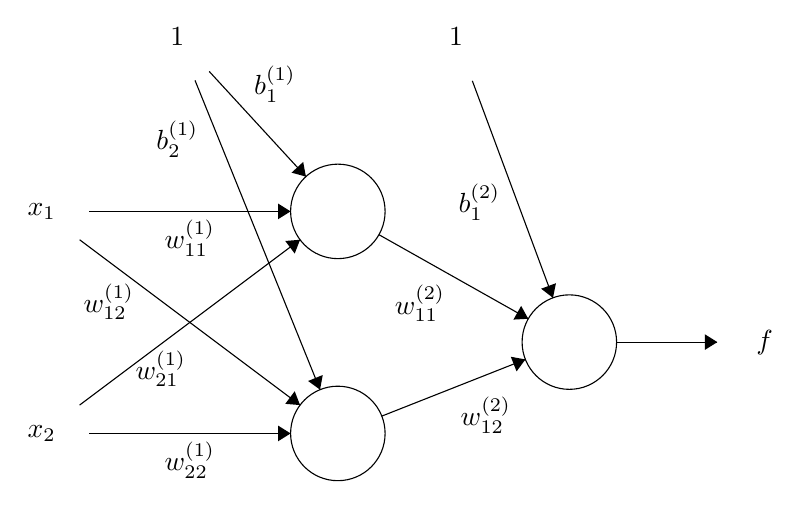
\begin{tikzpicture}[scale=0.2]
\tikzstyle{every node}+=[inner sep=0pt]
\draw [black] (34,-24.7) circle (3);
\draw [black] (34,-38.8) circle (3);
\draw [black] (48.7,-33) circle (3);
\draw (15.2,-24.7) node {$x_1$};
\draw (15.2,-38.8) node {$x_2$};
\draw (61.1,-33) node {$f$};
\draw (23.8,-13.6) node {$1$};
\draw (41.5,-13.6) node {$1$};
\draw [black] (36.79,-37.7) -- (45.91,-34.1);
\fill [black] (45.91,-34.1) -- (44.98,-33.93) -- (45.35,-34.86);
\draw (43.4,-36.44) node [below] {$w_{12}^{(2)}$};
\draw [black] (36.61,-26.18) -- (46.09,-31.52);
\fill [black] (46.09,-31.52) -- (45.64,-30.7) -- (45.15,-31.57);
\draw (39.21,-29.35) node [below] {$w_{11}^{(2)}$};
\draw [black] (17.6,-26.5) -- (31.6,-37);
\fill [black] (31.6,-37) -- (31.26,-36.12) -- (30.66,-36.92);
\draw (19.45,-29.25) node [below] {$w_{12}^{(1)}$};
\draw [black] (17.6,-37) -- (31.6,-26.5);
\fill [black] (31.6,-26.5) -- (30.66,-26.58) -- (31.26,-27.38);
\draw (22.75,-33.50) node [below] {$w_{21}^{(1)}$};
\draw [black] (51.7,-33) -- (58.1,-33);
\fill [black] (58.1,-33) -- (57.3,-32.5) -- (57.3,-33.5);
\draw [black] (25.83,-15.81) -- (31.97,-22.49);
\fill [black] (31.97,-22.49) -- (31.8,-21.56) -- (31.06,-22.24);
\draw (31.36,-16.61) node [left] {$b_1^{(1)}$};
\draw [black] (42.54,-16.41) -- (47.66,-30.19);
\fill [black] (47.66,-30.19) -- (47.85,-29.26) -- (46.91,-29.61);
\draw (44.34,-24.11) node [left] {$b_1^{(2)}$};
\draw [black] (24.93,-16.38) -- (32.87,-36.02);
\fill [black] (32.87,-36.02) -- (33.04,-35.09) -- (32.11,-35.47);
\draw (25.16,-20.1) node [left] {$b_2^{(1)}$};
\draw [black] (18.2,-24.7) -- (31,-24.7);
\fill [black] (31,-24.7) -- (30.2,-24.2) -- (30.2,-25.2);
\draw (24.6,-25.2) node [below] {$w_{11}^{(1)}$};
\draw [black] (18.2,-38.8) -- (31,-38.8);
\fill [black] (31,-38.8) -- (30.2,-38.3) -- (30.2,-39.3);
\draw (24.6,-39.3) node [below] {$w_{22}^{(1)}$};
\end{tikzpicture}
\caption{\label{fig:ex-backprop}Red neuronal sencilla de dos capas con entrada vectorial de dos componentes, se marcan los pesos y los sesgos en cada conexión}
\end{figure}

En este caso, el vector de parámetros que determina la red será
$$\theta=\left(w_{11}^{(1)},w_{12}^{(1)},w_{21}^{(1)},w_{22}^{(1)},b_{1}^{(1)},b_{2}^{(1)},w_{11}^{(2)},w_{12}^{(2)},b_{1}^{(2)}\right).$$
Puesto que la función de coste $J$ vendrá determinada por el valor de $f$ en el mismo punto, para calcular su gradiente nos interesa conocer el de $f$. La expresión desarrollada de $f$ queda
\begin{gather*}
f(x_1,x_2;\theta)=\\g\left(w_{21}^{(2)}g\left(w_{11}^{(1)}x_{1}+w_{12}^{(1)}x_2+b_1^{(1)}\right)+w_{22}^{(2)}g\left(w_{21}^{(1)}x_1+w_{22}^{(1)}x_2+b_2^{(1)}\right)+b_1^{(2)}\right).
\end{gather*}

Ahora, mediante la regla de la cadena podemos desarrollar la parcial de $f$ respecto de cualquiera de los parámetros. Llamamos
\begin{align*}
  \alpha&=g'\left(w_{21}^{(2)} g\left(w_{11}^{(1)}x_{1}+w_{12}^{(1)}x_2+b_1^{(1)}\right) + w_{22}^{(2)} g\left(w_{21}^{(1)}x_1+w_{22}^{(1)}x_2+b_2^{(1)}\right)+b_1^{(2)}\right)\\
  \beta&=g'\left(w_{11}^{(1)}x_{1}+w_{12}^{(1)}x_2+b_1^{(1)}\right)\\
  \gamma&=g'\left(w_{21}^{(1)}x_{1}+w_{22}^{(1)}x_2+b_2^{(1)}\right)
\end{align*}
y se tiene
\begin{alignat*}{3}
  \frac{\partial f}{\partial w_{11}^{(1)}}(x_1,x_2;\theta)&=\alpha w_{11}^{(2)}\beta x_1,\quad&
  \frac{\partial f}{\partial w_{12}^{(1)}}(x_1,x_2;\theta)&=\alpha w_{11}^{(2)}\beta x_2,\\
  \frac{\partial f}{\partial w_{21}^{(1)}}(x_1,x_2;\theta)&=\alpha w_{12}^{(2)}\gamma x_1,\quad&
  \frac{\partial f}{\partial w_{22}^{(1)}}(x_1,x_2;\theta)&=\alpha w_{12}^{(2)}\gamma x_2,\\
  \frac{\partial f}{\partial b_{1}^{(1)}}(x_1,x_2;\theta)&=\alpha w_{11}^{(2)}\beta, \quad&
  \frac{\partial f}{\partial b_{2}^{(1)}}(x_1,x_2;\theta)&=\alpha w_{12}^{(2)}\gamma, \\
  \frac{\partial f}{\partial w_{11}^{(2)}}(x_1,x_2;\theta)&=\alpha g(w_{11}^{(1)}x_{1}+w_{12}^{(1)}x_2 + b_1^{(1)}),&&\\
  \frac{\partial f}{\partial w_{12}^{(2)}}(x_1,x_2;\theta)&=\alpha g(w_{21}^{(1)}x_{1}+w_{22}^{(1)}x_2 + b_2^{(1)}),&\quad
  \frac{\partial f}{\partial b_{1}^{(2)}}(x_1,x_2;\theta)&=\alpha.
\end{alignat*}

Como podemos observar, algunos de los factores de las parciales se repiten en varias de ellas, de forma que se ahorrarán muchos cálculos innecesarios si no se repiten. Este hecho se hace aún más evidente conforme se añaden capas a la red y unidades a cada capa. Por ello, el algoritmo de propagación hacia atrás permite optimizar el cálculo del gradiente mediante varios pasos intermedios para evitar cálculos repetidos.

\end{example}

En el algoritmo \ref{alg:backprop} se describe \emph{backprop} paso a
paso. Es fácil comprobar que aplicando esta técnica al ejemplo anterior
podemos evaluar las parciales que se han deducido sin repetir cálculos
costosos.

\begin{algorithm}
\caption{Propagación hacia atrás}
\label{alg:backprop}
\begin{algorithmic}
\STATE{Tras la propagación hacia adelante, calcular el gradiente de la capa de salida:}
\STATE{$d\gets \nabla_{y}J(y,y^{*};\theta)=\nabla_{y}L(y,y^{*})$}
  \FOR{$k=l,\dots,1$}
  \STATE{Aplicar la regla de la cadena a la función de activación ($\odot$ denota producto componente a componente):}
  \STATE{$d\gets \nabla_{z^{(k)}}J=d\odot g'(z^{i})$}
  \STATE{Calcular gradientes en los pesos y sesgos (incluyendo el término de regularización si es necesario):}
  \STATE{$\nabla_{b^{(k)}}J=d+\lambda\nabla_{b^{(k)}}\Omega(\theta)$}
  \STATE{$\nabla_{W^{(k)}}J=d\Tr{(h^{(k-1)})}+\lambda\nabla_{W^{(k)}}\Omega(\theta)$}
  \STATE{Propagar el gradiente hacia la capa oculta anterior:}
  \STATE{$d\gets \nabla_{h^{(k-1)}}J=\Tr{(W^{(k)})}d$}
  \ENDFOR
\end{algorithmic}
\end{algorithm}

\section{Optimización en Deep
Learning}\label{optimizaciuxf3n-en-deep-learning}

\label{sec:dl-opt}

\subsection{Gradiente descendiente estocástico
(SGD)}\label{gradiente-descendiente-estocuxe1stico-sgd}

En aprendizaje automático, y especialmente en Deep Learning, es común
utilizar conjuntos de datos con un gran número de instancias, para
favorecer la capacidad de generalización de los modelos producidos por
algoritmos. Esto provoca que el coste computacional de calcular cada
paso de un gradiente descendente haga inviable su uso. Sin embargo, se
puede utilizar una aproximación estocástica al algoritmo denominada
gradiente descendiente estocástico (\emph{Stochastic Gradient Descent},
SGD). En esta versión de gradiente descendiente se asienta la mayor
parte del desarrollo del Deep Learning en la actualidad.

Al ser una aproximación estocástica, SGD calcula un estimador del
gradiente de la función objetivo a partir de un número reducido de
muestras. Se describe en el algoritmo \ref{alg:sgd}.

\begin{algorithm}
\caption{Gradiente descendiente estocástico, iteración $k$-ésima}
\label{alg:sgd}
\begin{algorithmic}
  \REQUIRE{Tasa de aprendizaje $\varepsilon_k$}
  \REQUIRE{Parámetro inicial $\theta$}
  \WHILE{no se alcanza criterio de parada}
  \STATE{Escoger un minilote de $m$ instancias del conjunto de entrenamiento $x^{(1)},\dots,x^{(m)}$ con correspondientes objetivos $y^{(i)}$}
  \STATE{Calcular estimador del gradiente: $\hat g\gets \frac 1 m \nabla \sum_i L(f(x^{(i)}; \theta),y^{(i)})$}
  \STATE{Actualizar parámetro: $\theta\gets\theta - \varepsilon_k\hat g$}
  \ENDWHILE
\end{algorithmic}
\end{algorithm}

\subsection{Variantes de SGD}\label{variantes-de-sgd}

\subsubsection{SGD con momento}\label{sgd-con-momento}

El momento es un término adicional que fuerza a que SGD varíe menos la
dirección de una iteración a otra. De esta forma, el zigzagueo
característico de GD, también presente en SGD, se atenúa. Esta versión
se describe en el algoritmo \ref{alg:sgdm}.

\begin{algorithm}
\caption{Gradiente descendiente estocástico con momento}
\label{alg:sgdm}
\begin{algorithmic}
  \REQUIRE{Tasa de aprendizaje $\varepsilon$, momento $\alpha$}
  \REQUIRE{Parámetro inicial $\theta$, velocidad inicial $v$}
  \WHILE{no se alcanza criterio de parada}
  \STATE{Escoger un minilote de $m$ instancias del conjunto de entrenamiento $x^{(1)},\dots,x^{(m)}$ con correspondientes objetivos $y^{(i)}$}
  \STATE{Calcular estimador del gradiente: $\hat g\gets \frac 1 m \nabla \sum_i L(f(x^{(i)}; \theta),y^{(i)})$}
  \STATE{Actualizar la velocidad: $v\gets\alpha v - \varepsilon \hat g$}
  \STATE{Actualizar parámetro: $\theta\gets\theta + v$}
  \ENDWHILE
\end{algorithmic}
\end{algorithm}

\subsubsection{AdaGrad}\label{adagrad}

Adagrad \autocite{adagrad} es una versión adaptativa de SGD, en el
sentido de que varía los parámetros de forma inversamente proporcional a
la raíz cuadrada de la suma de los cuadrados de los valores anteriores.
Así, en lugar de decrementar la tasa de aprendizaje de igual forma para
todos los parámetros, la decrementa más rápido en los parámetros que
tienen mayores derivadas parciales. Como resultado adicional, en las
zonas de menor pendiente del espacio de parámetros el algoritmo progresa
más rápidamente que SGD. Se describe en el algoritmo \ref{alg:adagrad}.

\begin{algorithm}
\caption{Adagrad}
\label{alg:adagrad}
\textbf{Notación:} $\odot$ es el producto componente a componente, $\sqrt{.}$ es la raíz cuadrada componente a componente y la división por $\frac{1}{\delta + \sqrt r}$ se realiza componente a componente.
\begin{algorithmic}
  \REQUIRE{Tasa de aprendizaje $\varepsilon$, constante pequeña $\delta$}
  \REQUIRE{Parámetro inicial $\theta$}
  \STATE{Inicializar: $r\gets 0$}
  \WHILE{no se alcanza criterio de parada}
  \STATE{Escoger un minilote de $m$ instancias del conjunto de entrenamiento $x^{(1)},\dots,x^{(m)}$ con correspondientes objetivos $y^{(i)}$}
  \STATE{Calcular estimador del gradiente: $\hat g\gets \frac 1 m \nabla \sum_i L(f(x^{(i)}; \theta),y^{(i)})$}
  \STATE{Acumular cuadrado del gradiente: $r\gets r + \hat g\odot \hat g$}
  \STATE{Calcular actualización: $\Delta\theta\gets - \frac{\varepsilon}{\delta + \sqrt{r}}\odot \hat g$}
  \STATE{Actualizar parámetro: $\theta\gets\theta + \Delta\theta$}
  \ENDWHILE
\end{algorithmic}
\end{algorithm}

\subsubsection{RMSProp}\label{rmsprop}

El algoritmo RMSProp, detallado en el algoritmo \ref{alg:rmsprop},
sustituye la acumulación de gradientes de AdaGrad por una media
exponencial, de forma que tenga mejor comportamiento al optimizar
funciones no convexas.

\begin{algorithm}
\caption{RMSProp}
\label{alg:rmsprop}
\textbf{Notación:} De nuevo, las operaciones $\odot$, raíz cuadrada y división se realizan componente a componente.
\begin{algorithmic}
  \REQUIRE{Tasa de aprendizaje $\varepsilon$, constante pequeña $\delta$}
  \REQUIRE{Tasa de decaimiento $\rho$}
  \REQUIRE{Parámetro inicial $\theta$}
  \STATE{Inicializar: $r\gets 0$}
  \WHILE{no se alcanza criterio de parada}
  \STATE{Escoger un minilote de $m$ instancias del conjunto de entrenamiento $x^{(1)},\dots,x^{(m)}$ con correspondientes objetivos $y^{(i)}$}
  \STATE{Calcular estimador del gradiente: $\hat g\gets \frac 1 m \nabla \sum_i L(f(x^{(i)}; \theta),y^{(i)})$}
  \STATE{Acumular cuadrado del gradiente: $r\gets \rho r + (1 - \rho) \hat g\odot \hat g$}
  \STATE{Calcular actualización: $\Delta\theta\gets - \frac{\varepsilon}{\sqrt{\delta + r}}\odot \hat g$}
  \STATE{Actualizar parámetro: $\theta\gets\theta + \Delta\theta$}
  \ENDWHILE
\end{algorithmic}
\end{algorithm}

\subsubsection{Adam}\label{adam}

Adam es un algoritmo que también adapta la tasa de aprendizaje y además
introduce un momento adaptativo, se puede considerar una combinación de
RMSProp con momento. Se describe en el algoritmo \ref{alg:adam}.

\begin{algorithm}
\caption{Adam}
\label{alg:adam}
\begin{algorithmic}
  \REQUIRE{Tasa de aprendizaje $\varepsilon$, constante pequeña $\delta$}
  \REQUIRE{Tasas de decaimiento exponencial $\rho_{1}, \rho_2\in[0,1[$}
  \REQUIRE{Parámetro inicial $\theta$}
  \STATE{Inicializar: $s\gets 0, r\gets 0, t\gets 0$}
  \WHILE{no se alcanza criterio de parada}
  \STATE{Escoger un minilote de $m$ instancias del conjunto de entrenamiento $x^{(1)},\dots,x^{(m)}$ con correspondientes objetivos $y^{(i)}$}
  \STATE{Calcular estimador del gradiente: $\hat g\gets \frac 1 m \nabla \sum_i L(f(x^{(i)}; \theta),y^{(i)})$}
  \STATE{Incrementar tiempo: $t\gets t + 1$}
  \STATE{Actualizar estimador sesgado del 1er momento: $s\gets \rho_1 s + (1 - \rho_1)\hat g$}
  \STATE{Actualizar estimador sesgado del 2º momento: $r\gets \rho_2 s + (1 - \rho_2)\hat g\odot \hat g$}
  \STATE{Corregir sesgos: $\hat s\gets\frac{s}{1 - \rho_1^t},\ \hat r\gets\frac{r}{1 - \rho_2^t}$}
  \STATE{Calcular actualización: $\Delta\theta\gets - \frac{\varepsilon}{\delta + \sqrt{\hat r}}\hat s$ (operaciones componente a componente)}
  \STATE{Actualizar parámetro: $\theta\gets\theta + \Delta\theta$}
  \ENDWHILE
\end{algorithmic}
\end{algorithm}

\section{Estructuras profundas no
supervisadas}\label{estructuras-profundas-no-supervisadas}

\subsection{Máquina de Boltzmann restringidas
(RBM)}\label{muxe1quina-de-boltzmann-restringidas-rbm}

\subsection{Autoencoder}\label{autoencoder}

\begin{figure}[hbtp]
  \centering
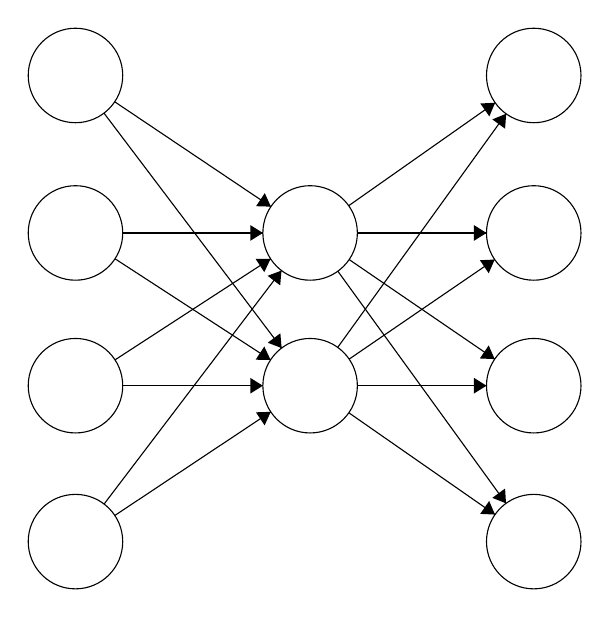
\begin{tikzpicture}[scale=0.2]
\tikzstyle{every node}+=[inner sep=0pt]
\draw [black] (21.5,-13.4) circle (3);
\draw [black] (21.5,-23.4) circle (3);
\draw [black] (21.5,-33.1) circle (3);
\draw [black] (36.4,-23.4) circle (3);
\draw [black] (36.4,-33.1) circle (3);
\draw [black] (50.6,-23.4) circle (3);
\draw [black] (21.5,-43) circle (3);
\draw [black] (50.6,-33.1) circle (3);
\draw [black] (50.6,-43) circle (3);
\draw [black] (50.6,-13.4) circle (3);
\draw [black] (24.5,-33.1) -- (33.4,-33.1);
\fill [black] (33.4,-33.1) -- (32.6,-32.6) -- (32.6,-33.6);
\draw [black] (24.01,-31.46) -- (33.89,-25.04);
\fill [black] (33.89,-25.04) -- (32.94,-25.05) -- (33.49,-25.89);
\draw [black] (24.5,-23.4) -- (33.4,-23.4);
\fill [black] (33.4,-23.4) -- (32.6,-22.9) -- (32.6,-23.9);
\draw [black] (24.01,-25.04) -- (33.89,-31.46);
\fill [black] (33.89,-31.46) -- (33.49,-30.61) -- (32.94,-31.45);
\draw [black] (23.99,-15.07) -- (33.91,-21.73);
\fill [black] (33.91,-21.73) -- (33.52,-20.87) -- (32.97,-21.7);
\draw [black] (23.31,-15.79) -- (34.59,-30.71);
\fill [black] (34.59,-30.71) -- (34.51,-29.77) -- (33.71,-30.37);
\draw [black] (39.4,-23.4) -- (47.6,-23.4);
\fill [black] (47.6,-23.4) -- (46.8,-22.9) -- (46.8,-23.9);
\draw [black] (38.88,-31.41) -- (48.12,-25.09);
\fill [black] (48.12,-25.09) -- (47.18,-25.13) -- (47.74,-25.96);
\draw [black] (24,-41.34) -- (33.9,-34.76);
\fill [black] (33.9,-34.76) -- (32.96,-34.79) -- (33.51,-35.62);
\draw [black] (23.32,-40.61) -- (34.58,-25.79);
\fill [black] (34.58,-25.79) -- (33.7,-26.12) -- (34.5,-26.73);
\draw [black] (38.85,-21.67) -- (48.15,-15.13);
\fill [black] (48.15,-15.13) -- (47.21,-15.18) -- (47.78,-16);
\draw [black] (38.88,-25.09) -- (48.12,-31.41);
\fill [black] (48.12,-31.41) -- (47.74,-30.54) -- (47.18,-31.37);
\draw [black] (38.16,-25.83) -- (48.84,-40.57);
\fill [black] (48.84,-40.57) -- (48.78,-39.63) -- (47.97,-40.22);
\draw [black] (38.15,-30.67) -- (48.85,-15.83);
\fill [black] (48.85,-15.83) -- (47.97,-16.19) -- (48.78,-16.78);
\draw [black] (39.4,-33.1) -- (47.6,-33.1);
\fill [black] (47.6,-33.1) -- (46.8,-32.6) -- (46.8,-33.6);
\draw [black] (38.86,-34.82) -- (48.14,-41.28);
\fill [black] (48.14,-41.28) -- (47.77,-40.42) -- (47.2,-41.24);
\end{tikzpicture}
\caption{\label{fig:autoencoder}Autoencoder de tres capas} 
\end{figure}

\textcite{hinton2006autoencoder}

\subsection{Entrenamiento de
autoencoders}\label{entrenamiento-de-autoencoders}

\subsubsection{Pre-entrenamiento}\label{pre-entrenamiento}

\subsubsection{Ajuste fino}\label{ajuste-fino}
